\section{Coherences and their interactions}
\paragraph{Formation and autonomy.} A detector requiring an isolated core of width at most 8 that
persists for 64 ticks (confirmed on a larger ring) found \ncoreSingle{} rules in which a single
event produces such a core, and \ncoreRules{} rules (\ncorePairs{} rule--seed pairs) with seeds of
up to four bits. Most of these move at the causal limit. To separate genuine objects from features
of larger structures we cut each mature core out, including both time layers, and re-ran it alone in
the matched vacuum. \nautSub{} of \nautSubN{} slower-than-light cores (\nautRules{} rules) survived
unchanged, compared with \nautLight{} of \nautLightN{} light-speed cores (Fig.~\ref{fig:objects}). Typical
speeds are $1/2$ and $1/3$. A frozen hypothesis that slow objects require an active vacuum was
\emph{falsified} by an exhaustive two-layer seed search: \nsilentSub{} silent-vacuum rules host
slow bounded objects, compared with \nactiveSub{} active-vacuum rules.

\begin{figure}[t]\centering
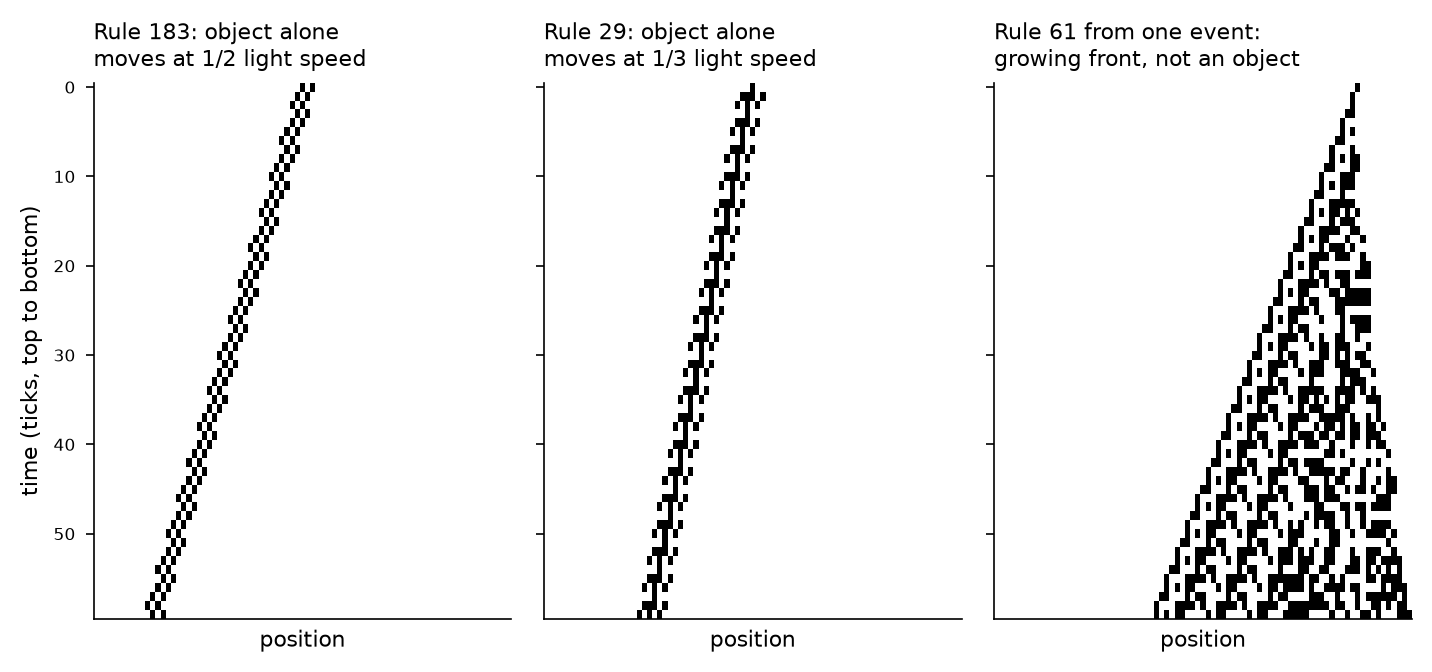
\includegraphics[width=\linewidth]{figures/fig1_objects.png}
\caption{Autonomous coherences cut out of their surroundings and run alone. Left and centre:
slower-than-light objects in rules 183 and 29. Right: a single event in rule 61 produces a growing
front, not an object. Time runs downward.}\label{fig:objects}
\end{figure}

\paragraph{Collisions.} Head-on collisions of the lowest-seed right- and left-moving objects
(\nctwoN{} collisions in \nctwoRules{} rules, eight impact phases each, all verified to make
contact) gave \nctwoElastic{} elastic outcomes, \nctwoTrans{} in which two different species
leave at the incoming speeds, \nctwoSup{} exact superpositions, \nctwoBubble{} in which the
collision opens an expanding domain of the opposite vacuum phase, and \nctwoUnres{} unresolved
outcomes. None annihilated, as reversibility requires (Fig.~\ref{fig:collisions}). In this design
every pair had opposite speeds of equal magnitude, so momentum-like conservation could not be tested.
Bubbles occurred only in active-vacuum rules, as predicted before the run.

\begin{figure}[t]\centering
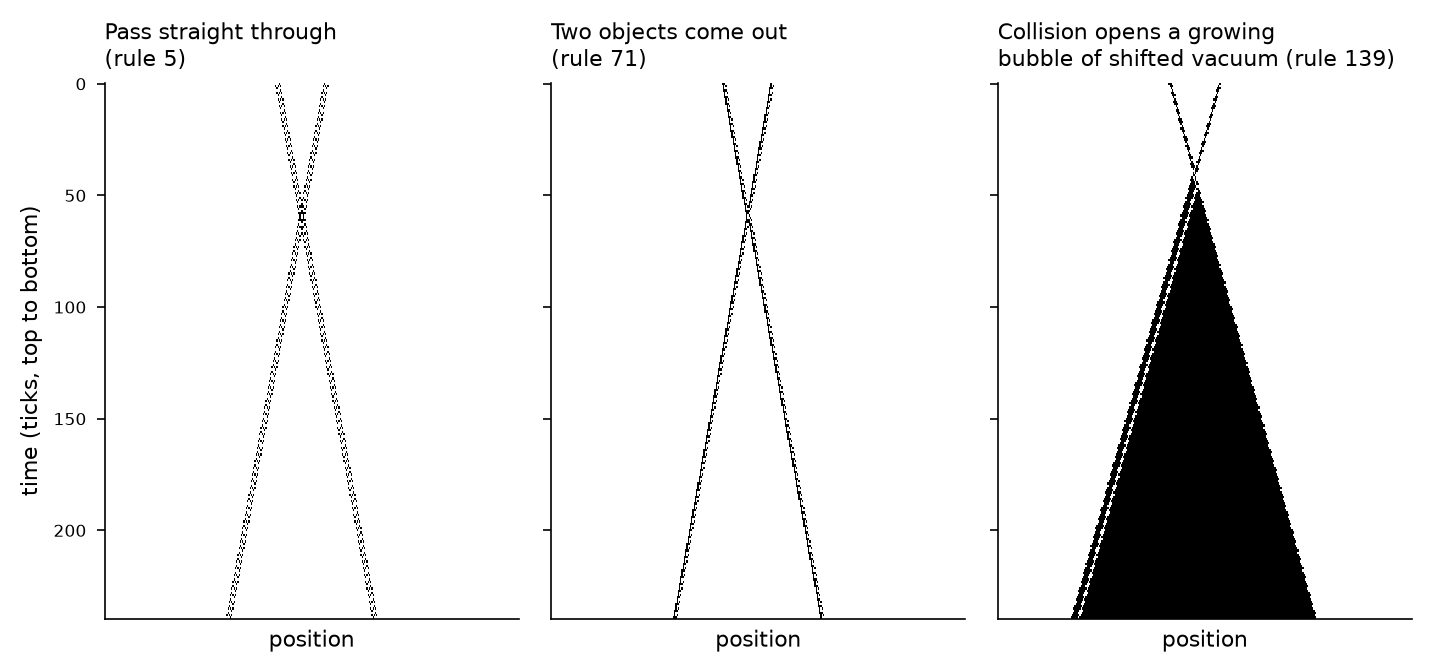
\includegraphics[width=\linewidth]{figures/fig2_collisions.png}
\caption{Three collision outcomes: exact pass-through, two coherences out, and a collision that
opens a growing domain of the opposite vacuum phase (black).}\label{fig:collisions}
\end{figure}
